\chapter{Evaluation}
\label{chap:evaluation}

To evaluate map-merging algorithm introduced in section~\ref{chap:mergingalgorithm} and to test performance of implemented map-merging node described in section~\ref{sec:map_merge-package}, I used $2$ data sources. First source are data from  simulation running several P3DX robots. Map-merging node was running through the whole exploring session testing online behaviour of the algorithm. Second data source are maps produced by \gls{SLAM} on \gls{MIT} Stata Center dataset presented in~\cite{Fallon2013}. \gls{MIT} dataset is produced by a single PR2 robot starting from different locations. Although this data does not come from multi-robot mapping, it is possible to test offline merging performance.

\section{Simulation setup}

I used \gls{VREP} simulator for experiment. All simulated robots were Pioneers P3-DX, which formed a homogeneous exploring team. Robots were setup using \texttt{p3dx\_robot} package available at~\cite{GitHubRoboRescue}, which also configures \gls{SLAM} and navigation for robots. Robots were using the \texttt{hector\_slam} package~\cite{2013:RoboCup} providing \gls{SLAM} algorithm and \texttt{move\_base} package~\cite{Marder2016}, part of the \gls{ROS} navigation stack, providing navigation for robots.

Cluster of 5 computers was formed to run simulator, robots, map-merging and exploring nodes. \gls{ROS} network was configured across all workstations using a single \gls{ROS} master running \texttt{roscore}. Every robot was using its own \gls{ROS} namespace for topics and was using a prefix for published \texttt{tf} frames to allow running multiple robots under the same \gls{ROS} master. This setup is well supported in \texttt{p3dx\_robot} package.

While \gls{VREP} is powerful and feature-rich simulator, its usage for multi-robot simulation have some limitations. First of all, \gls{VREP} support for headless mode (running without graphical environment) is not complete. Virtual framebuffer or similar technology is required, which adds performance overhead. Further \gls{VREP} does not scale properly to large number of threads, limiting number of robots for which simulation runs at bearable speed. For this reason it wasn't possible  to test more than 4 robots with this setup.

\section{\gls{MIT} dataset}
\label{sec:mit-dataset}

\gls{MIT} dataset are data available online in the form of rosbags~\cite{Fallon2013}. Data comes from mapping multi-floor \gls{MIT} building with PR2 robot. I have used only datasets from the second floor.

For all rosbags I have created maps using the \texttt{hector\_slam} package. It is the same \gls{SLAM} algorithm, which was used in simulation. This resulted in $36$ occupancy grid maps with sizes ranging from $2048 \times 2048$ cells to $5585 \times 4895$ cells.

Produced maps has been statically served in \gls{ROS} with running map-merging node. This setup is therefore limited to test offline merging, but allows a greater number of maps to participate in merging.

It is important to note that presented maps has been created by a single robot in a multi-session mapping. It is not a result of multi-robot mapping, although the robot initial positions vary between sessions and produced maps are similar to maps we would expect from multi-robot mapping.

\section{Merging with known initial positions}
\label{sec:merging-with-known-initial-positions}

Presented merging node can work with both known and unknown initial positions of robots. In the fist case the node uses initial positions to obtain transformation between grids. This setup was used in this experiment. Maps in this mode are not required to have any overlapping area.

Simulation scene is shown in figure~\ref{fig:minimal-overlapping-area-scene}. Figure~\ref{fig:merging-with-known-initial-positions-begin} shows initial maps, figure~\ref{fig:merging-with-known-initial-positions-end} shows maps after simulation ended. Note that figures~\ref{fig:merging-with-known-initial-positions-begin}, \ref{fig:merging-with-known-initial-positions-end} shows maps rotated compared to figure~\ref{fig:minimal-overlapping-area-scene}.

Video capturing map-merging during whole simulation, rosbag with map topics, scene with $3$ robots for \gls{VREP} simulator and full quality graphics are attached.

\begin{figure}
    \centering
    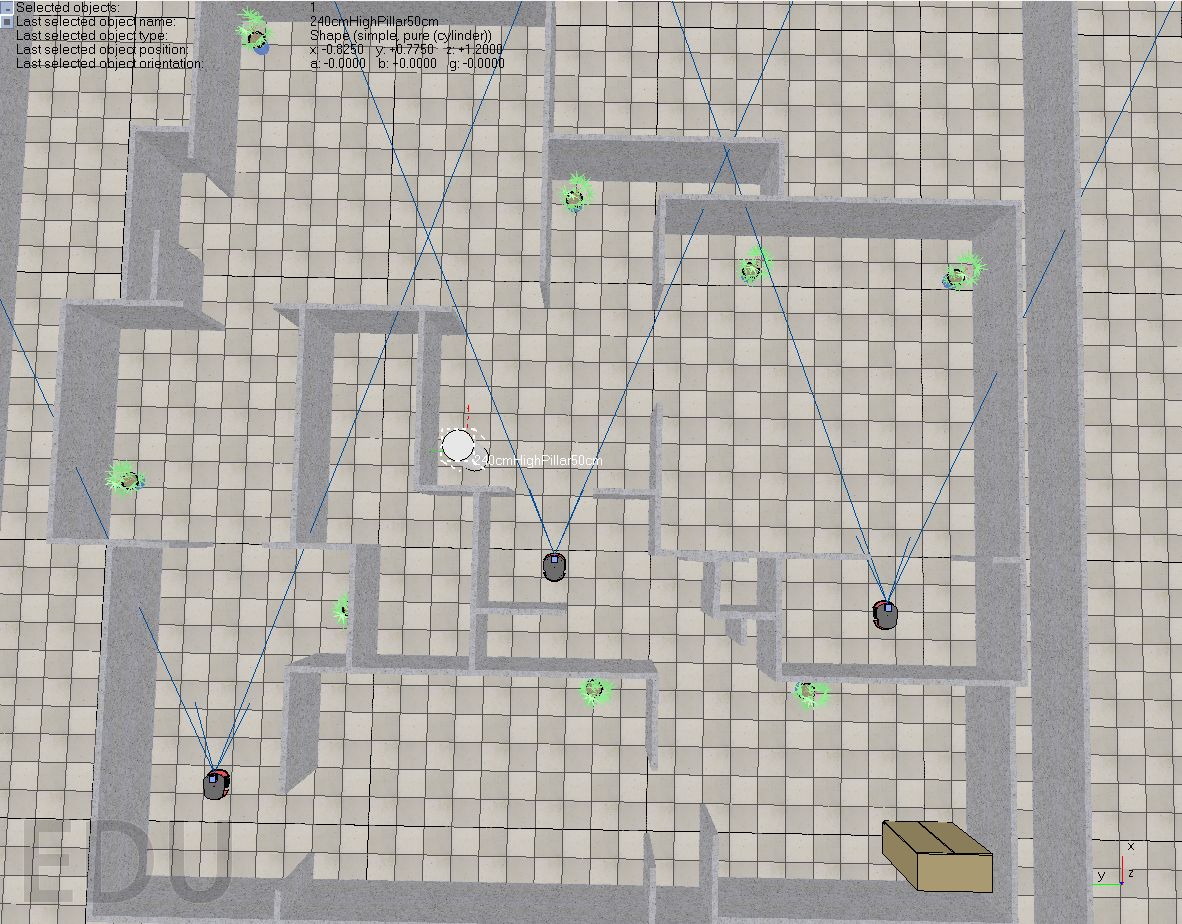
\includegraphics[width=3.93in]{../img/minimal-overlapping-area-scene.png}
    \caption{Scene for experiment with $3$ robots in \gls{VREP} simulator. Robot positions in scene are used as initial positions of robots for experiment.}
    \label{fig:minimal-overlapping-area-scene}
\end{figure}

\begin{figure}
    \centering
    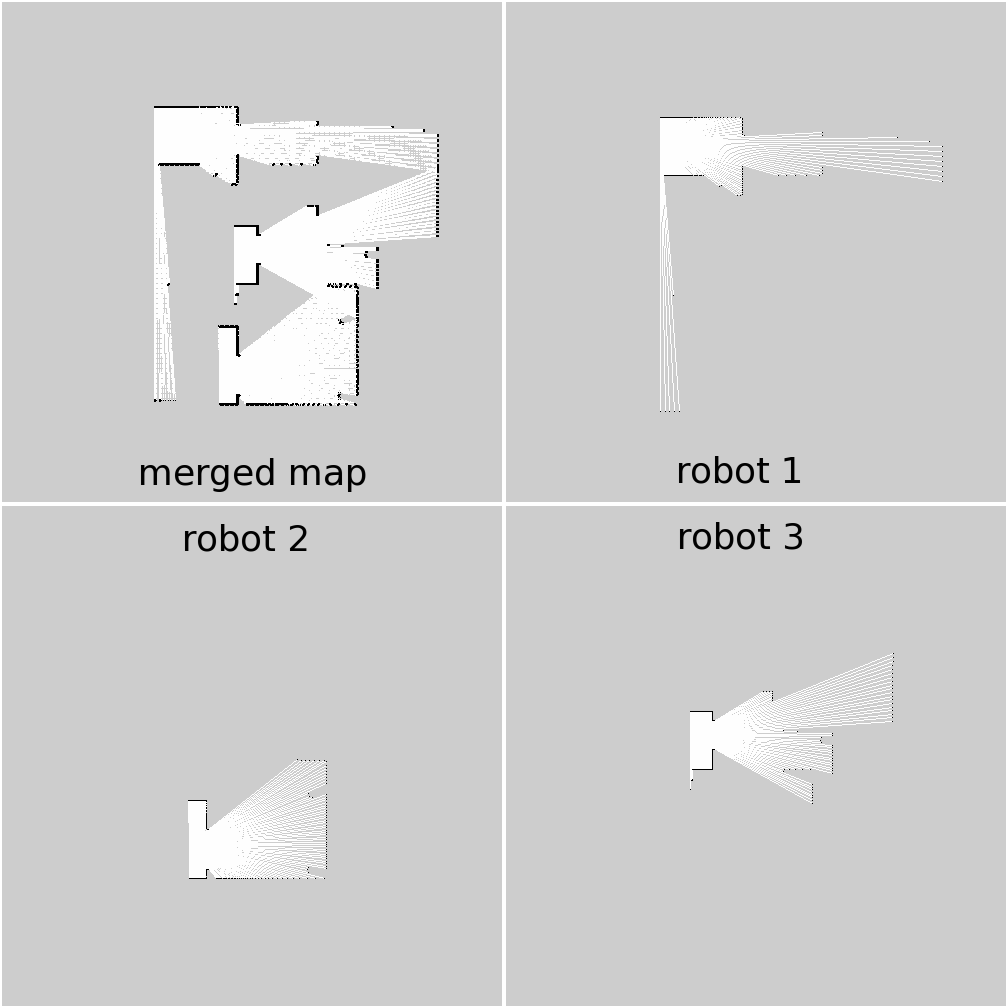
\includegraphics[width=3.35in]{../img/merging-with-known-initial-positions-begin.png}
    \caption{Initial maps produced by robots during experiment in simulator. Merged map is produced with knowledge of initial positions and can be therefore produced even without overlapping areas. In this situation merged map can be sparse.}
    \label{fig:merging-with-known-initial-positions-begin}
\end{figure}

\begin{figure}
    \centering
    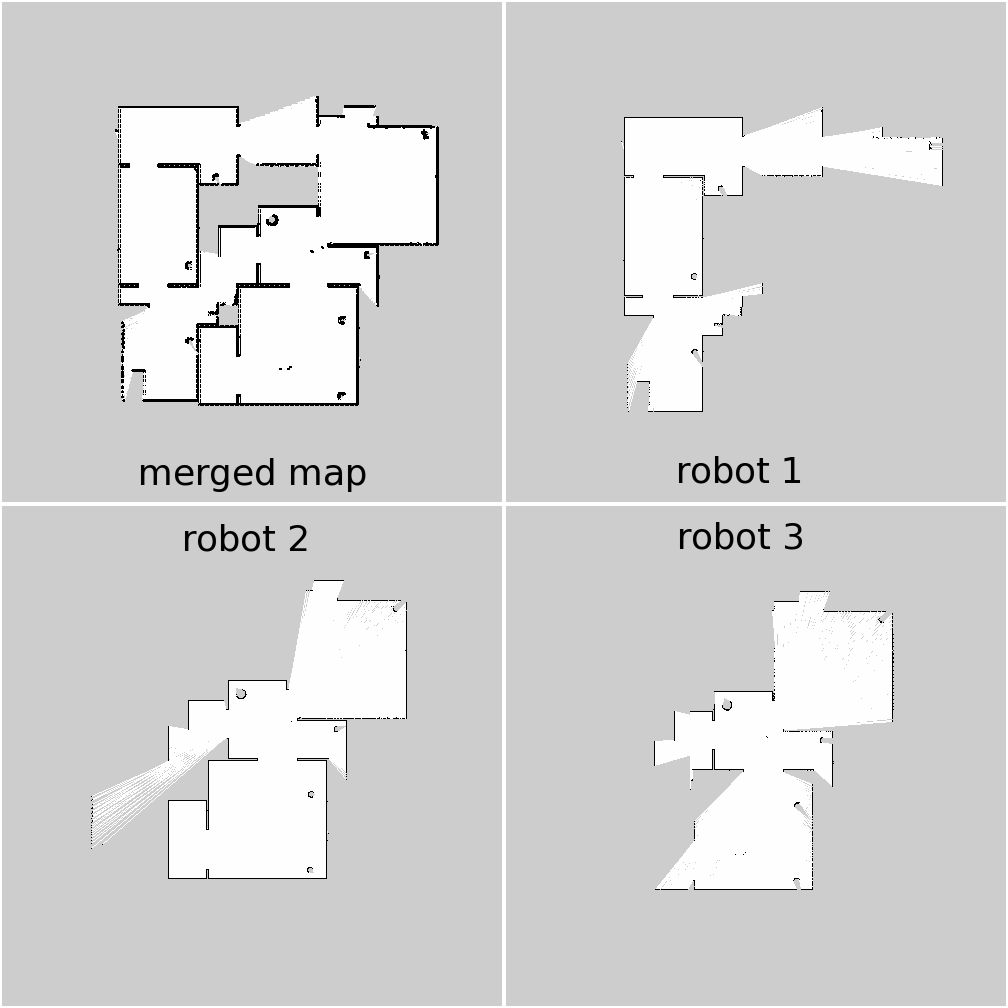
\includegraphics[width=3.35in]{../img/merging-with-known-initial-positions-end.png}
    \caption{Final maps produced in simulator. Merged map is produced with knowledge of initial positions.}
    \label{fig:merging-with-known-initial-positions-end}
\end{figure}

\section{Minimal overlapping area}
\label{sec:minimal-overlaping-area}

Map-merging algorithm presented in section~\ref{chap:mergingalgorithm} relies on overlapping areas of occupancy grids to produce a merged map. Minimal overlapping area to produce a reliable merge depends on environment being explored. Areas with high number of features in occupancy grids require small overlaps and vice versa.

Experiments showed that a reliable merge requires only about $90$ inliers, sometimes only $80$ inliers is enough to produce a correct transformation as seen in excerpt~\ref{fig:minimal-overlapping-area-log}. This excerpt is from the log of map-merging node presented in section~\ref{sec:map_merge-package} acquired during simulation.

Full log containing number of matches and number of inliers required to produce a transformation along with other details is available in the attachments. Scene for \gls{VREP} simulator, merged map and maps produced by robots are also attached. Maps has been taken as screenshots in rviz visualiser.

\begin{figure}
    \centering
	\begin{code}
AffineMatcher: have 121 matches
estimate:
[1.002576035215622, 0.00299917716022613, 62.49276756175958;
 -0.00299917716022613, 1.002576035215622, -240.2015971108993]
num_inliers 83
AffineMatcher: have 147 matches
estimate:
[1.002175802299877, -0.0004136975345276905, -15.26120294301828;
 0.0004136975345276905, 1.002175802299877, -120.7595895934327]
num_inliers 95
AffineMatcher: have 193 matches
estimate:
[1.000933706668138, 0.001232315845354937, 78.01218357952351;
 -0.001232315845354937, 1.000933706668138, -119.6792960984003]
num_inliers 157
	\end{code}
    \caption{Excerpt from the attached log of map-merging node captured during simulation. Shows output of matching phase of the algorithm for $3$ pairwise matches along with number of inliers.}
    \label{fig:minimal-overlapping-area-log}
\end{figure}


Simulation featured $3$ robots exploring common area. Figure~\ref{fig:minimal-overlapping-area-scene} shows the scene used in the experiment and initial robots positions. Figure~\ref{fig:minimal-overlapping-area-final-maps} shows maps produced by \gls{SLAM} after mapping finished. Figure~\ref{fig:minimal-overlapping-area-merged-map} shows the merged map produced by a map-merging node with unknown initial positions.

Simulation showed that a reliable merge between maps can be produced for $5-6$ overlapping rooms. After transformation is estimated, produced map is comparable to the reference map.

\begin{figure}
    \centering
    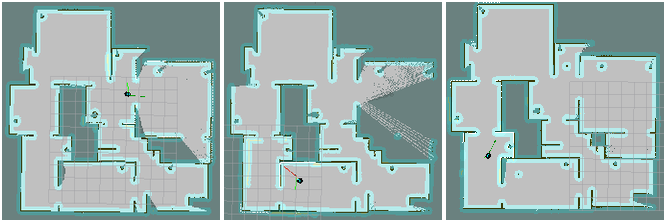
\includegraphics[width=2.22in]{../img/minimal-overlapping-area-final-maps.png}
    \caption{Maps produced by a multi-robot mapping in the simulator. Simulated scene can be seen in figure~\ref{fig:minimal-overlapping-area-scene}. Positions of the robots are final positions where robots finished mapping.}
    \label{fig:minimal-overlapping-area-final-maps}
\end{figure}

\begin{figure}
    \centering
    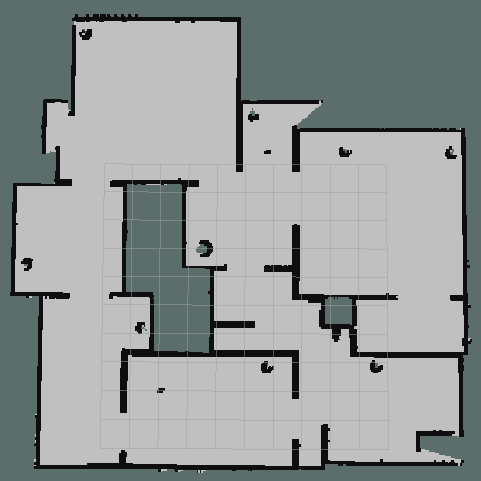
\includegraphics[width=1.58in]{../img/minimal-overlapping-area-merged-map.png}
    \caption{Merged map produced by the map-merging node. This map has been produced from $3$ maps shown in figure~\ref{fig:minimal-overlapping-area-final-maps}.}
    \label{fig:minimal-overlapping-area-merged-map}
\end{figure}

\section{Retaining largest transformation}
\label{sec:retaining-largest-transformation}

During online merging the merging algorithm presented in section~\ref{chap:mergingalgorithm} is launched repeatedly on growing grids. It might seem natural to preserve the transformation between largest number of grids. If the algorithm was able to produce a merge between $n$ grids in one point of time, it might seem like a good idea to preserve this transformation and use it for merging grids when the transformation is estimated for less than $n$ grids.

Experiments showed that this approach produce worse results than approach always using the newest transformation. Largest transformation retaining behaviour is problematic when there is not enough overlapping area between grids. Experiment presented in section~\ref{sec:merging-with-known-initial-positions} have maps that have very small overlaps.

Map-merging with unknown initial positions with largest transformation retaining launched in the same experiment as presented in section~\ref{sec:merging-with-known-initial-positions} shows the key problem of a such approach. Problem occurs when incorrect merge is produced due to too small overlaps. As shown in figure~\ref{fig:retaining-largest-transformation-montage}, incorrect unstable transformations, which are usually corrected quickly with small maps changes, are preserved due to largest transformation retaining after the estimation algorithm is no longer producing incorrect transformation. Incorrect transformations can be preserved for a long period of time with largest transformation retaining behaviour, when there is not enough overlapping area in the maps, so the incorrect transformation can be replaced with correct larger transformation.

Based on this and others experiments largest transformation retaining behaviour has been removed from map-merging node presented in section~\ref{sec:map_merge-package}.

Data for this experiment including rosbag with map topics, scene for \gls{VREP} simulator and presented maps are available in the attachments.

\begin{figure}
    \centering
    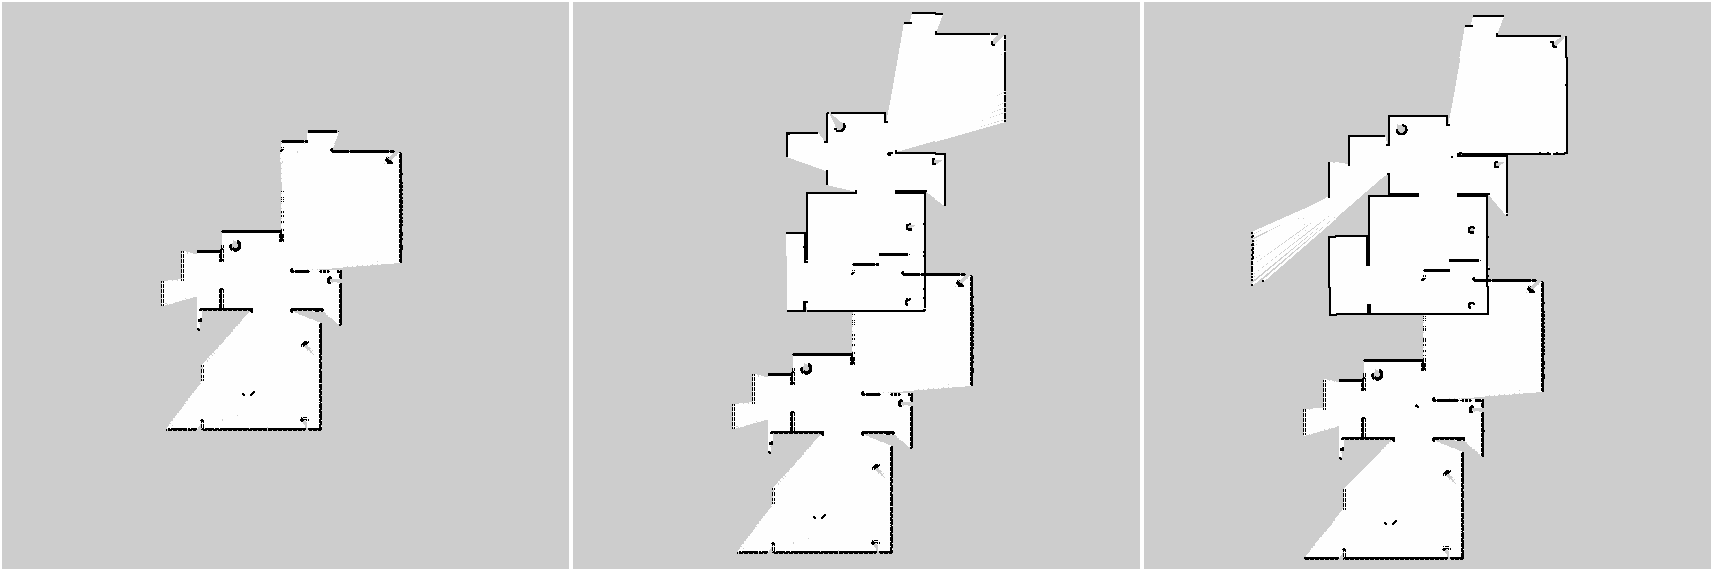
\includegraphics[width=5.71in]{../img/retaining-largest-transformation-montage.png}
    \caption{Map-merging with largest transformation retaining. From the left: Maps have no overlaps, unable to merge more than a single map. Incorrect transformation estimated due to too small overlaps. Overlapping space is still too small to produce a merge, but incorrect transformation was rejected. Due to largest transformation retaining incorrect merge is still produced.}
    \label{fig:retaining-largest-transformation-montage}
\end{figure}

\section{Probability model evaluation}
\label{sec:probability-model-evaluation}

Data from \gls{MIT} dataset are complex and difficult for \gls{SLAM} to produce a map without errors. In some cases overlapping areas does not exists. Such data are therefore suitable to test capabilities of map merging node to reject incorrect or non-mergeable maps.

Figure~\ref{fig:probability-model-evaluation-montage} shows $36$ maps obtained from \gls{MIT} dataset, all of them are from second floor. Empty maps are caused by \gls{SLAM} node failure. Note that maps contain many errors, some of them are completely broken as \gls{SLAM} localization failed. \texttt{hector\_slam} node uses only scans from base-mounted laser, better results might be achieved with different \gls{SLAM} approaches using stereo cameras and 3D scanning.

\begin{figure}
    \centering
    \includegraphics[width=\textwidth]{../img/mit-dataset-montage.png}
    \caption{$36$ maps created by \texttt{hector\_slam} from \gls{MIT} dataset.}
    \label{fig:probability-model-evaluation-montage}
\end{figure}

Merging algorithm uses thresholding described in section~\ref{sec:findinglargestconnectedcomponent} based on probabilistic model to reject low-confident matches. I have experimented with confidence threshold, which directly affects which matches will be present in merging (matches with low confidence are not considered). Figures~\ref{fig:probability-model-evaluation-treshold_1.0-12maps}, \ref{fig:probability-model-evaluation-treshold_1.5-9maps} and \ref{fig:probability-model-evaluation-treshold_2.0-3maps} show maps merged with confidence thresholds $1.0$, $1.5$ and $2.0$ respectively. Note that number of maps included in the merged map goes from $12$ to $3$.

Experiment has showed that increasing the confidence threshold to values greater that $1.0$ may lead to better results when maps are difficult to merge. Increasing threshold decreases number of maps merged significantly.

Data used for this experiment are available in the attachments. This data consist of maps produced by \gls{SLAM} on \gls{MIT} dataset and merged maps for tested thresholds. Raw data of \gls{MIT} dataset are available online~\cite{Fallon2013}.

\begin{figure}
    \centering
    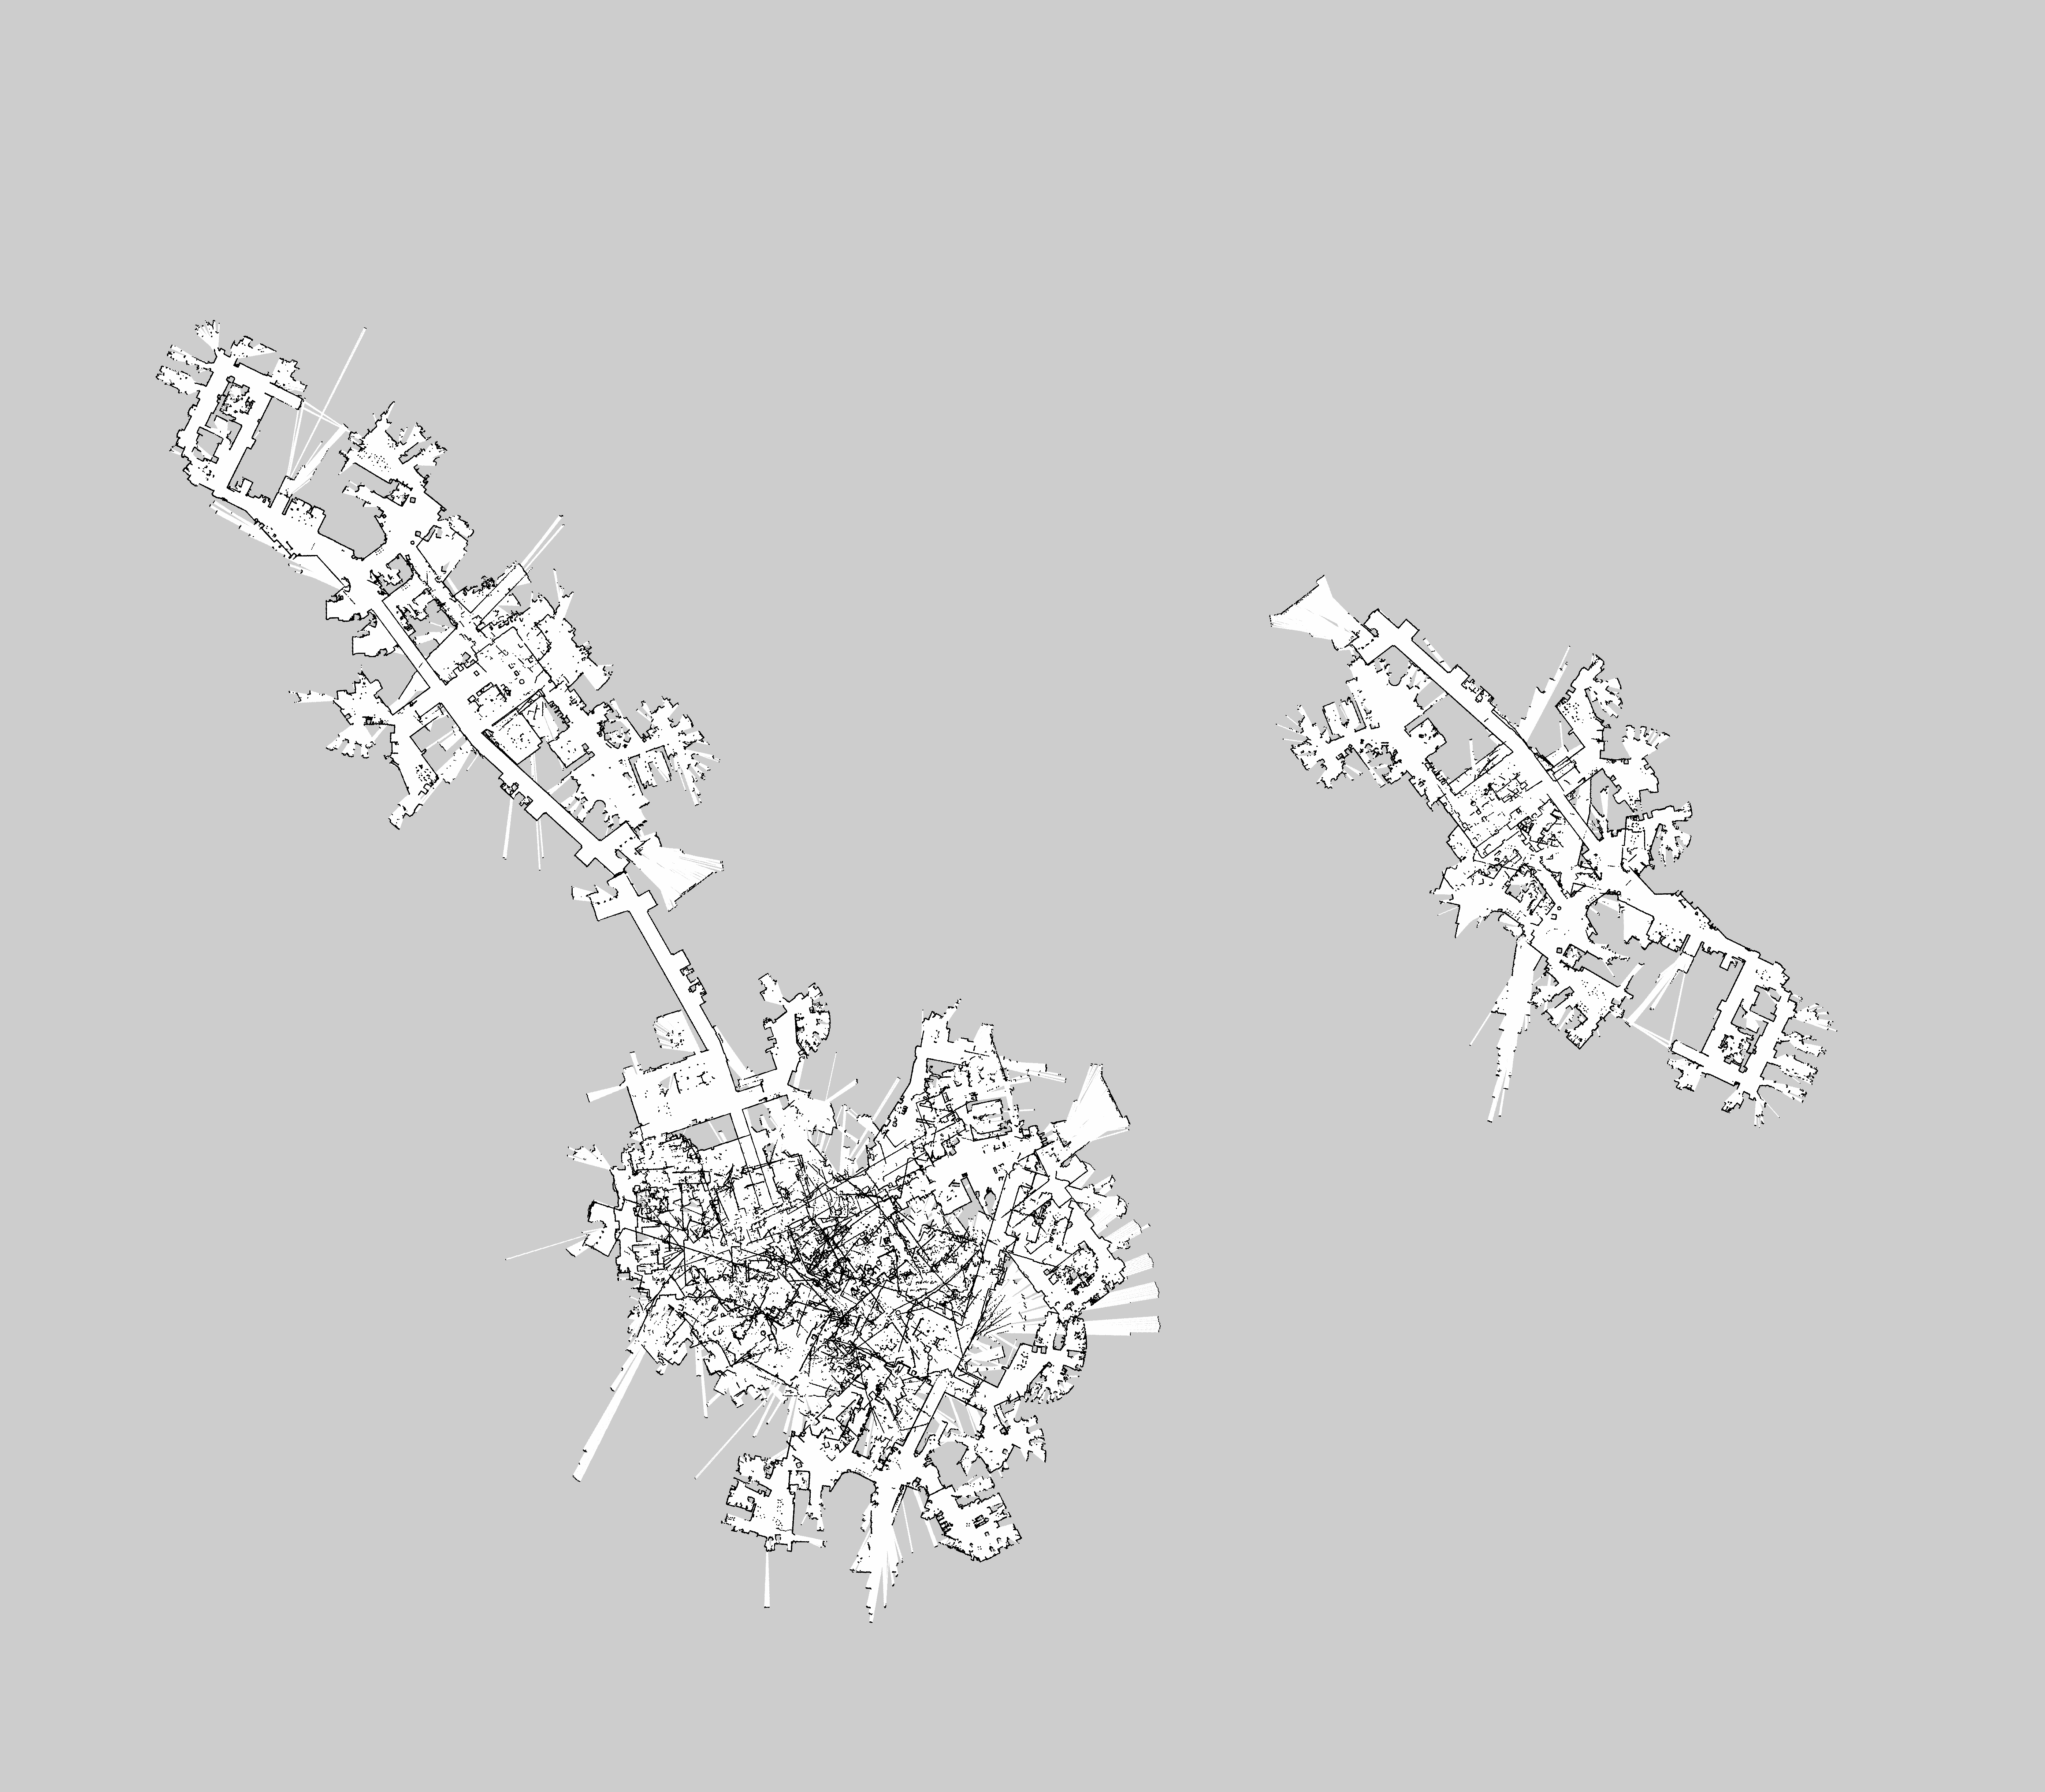
\includegraphics[width=\textwidth]{../img/probability-model-evaluation-treshold_1_0-12maps.png}
    \caption{Merged map created from $36$ maps shown in figure~\ref{fig:probability-model-evaluation-montage}. $12$ maps are included in the merged map. Confidence threshold is set to $1.0$.}
    \label{fig:probability-model-evaluation-treshold_1.0-12maps}
\end{figure}
\begin{figure}
    \centering
    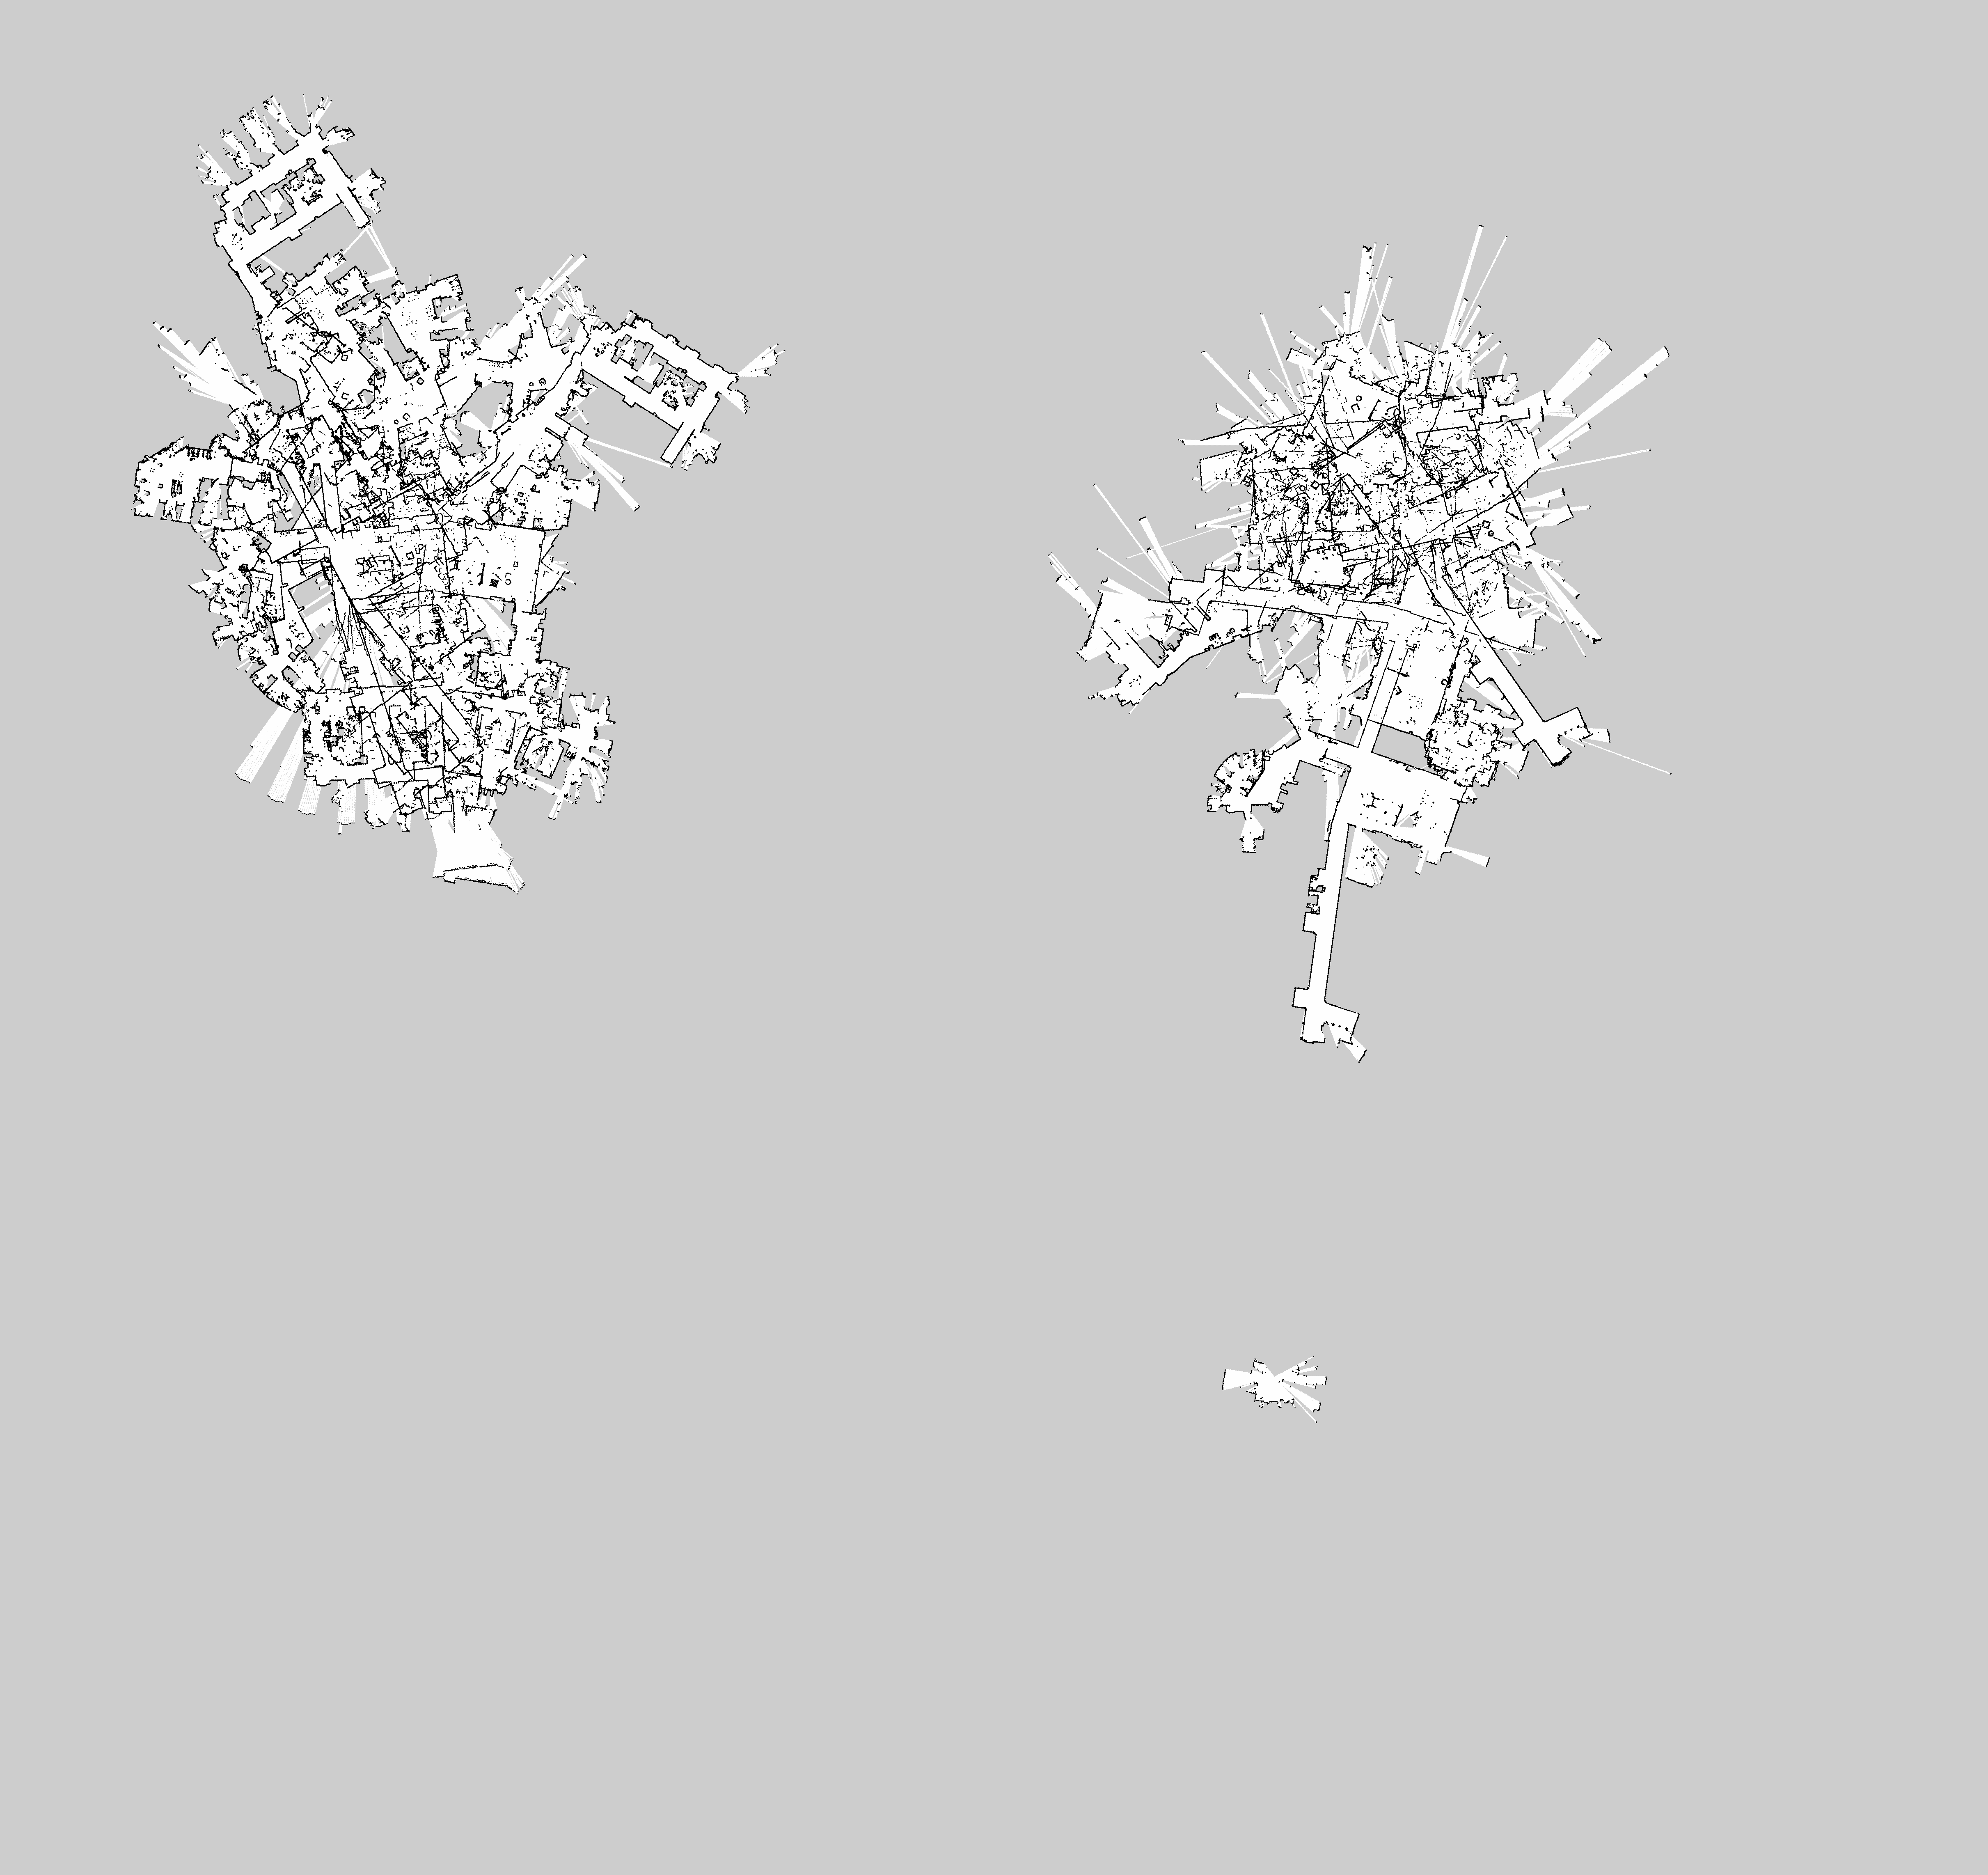
\includegraphics[width=\textwidth]{../img/probability-model-evaluation-treshold_1_5-9maps.png}
    \caption{Merged map created from $36$ maps shown in figure~\ref{fig:probability-model-evaluation-montage}. $9$ maps are included in the merged map. Confidence threshold is set to $1.5$.}
    \label{fig:probability-model-evaluation-treshold_1.5-9maps}
\end{figure}
\begin{figure}
    \centering
    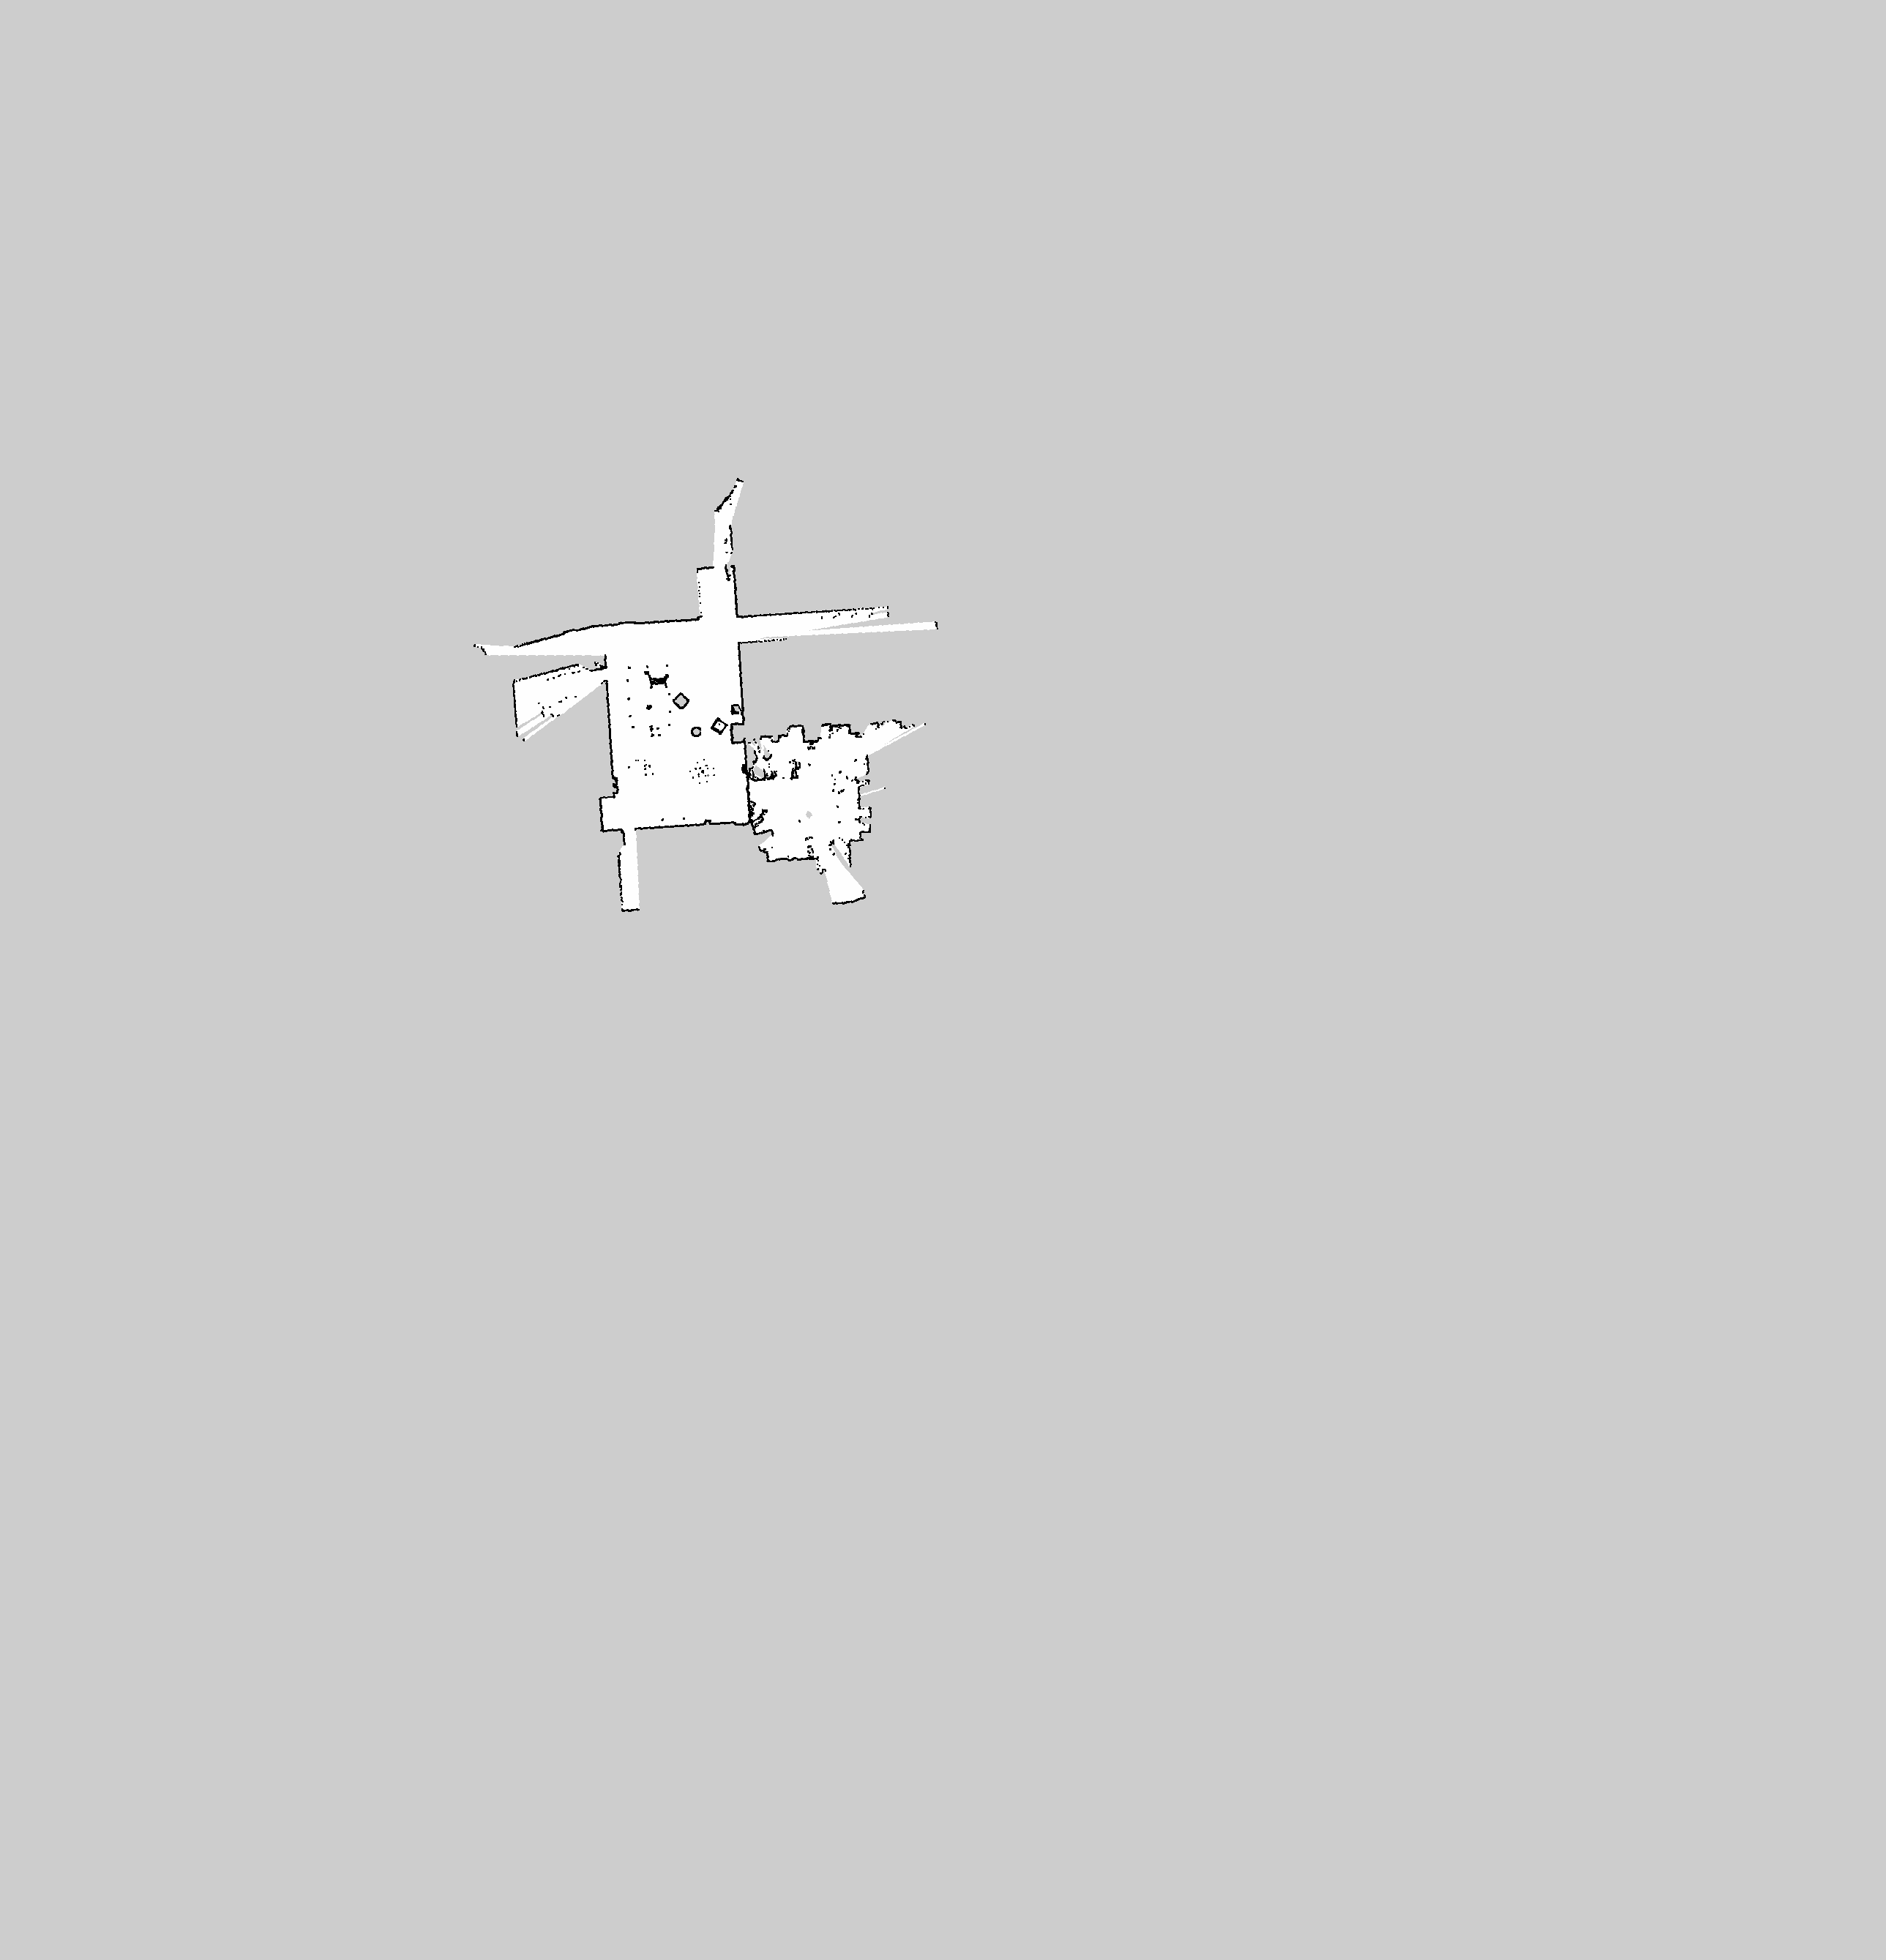
\includegraphics[width=\textwidth]{../img/probability-model-evaluation-treshold_2_0-3maps.png}
    \caption{Merged map created from $36$ maps shown in figure~\ref{fig:probability-model-evaluation-montage}. $3$ maps are included in the merged map. Confidence threshold is set to $2.0$.}
    \label{fig:probability-model-evaluation-treshold_2.0-3maps}
\end{figure}

% TODO:
% 3-robots evo 2 - rozbity slam
